\section{Räumliche Faltung}
\label{raeumliche_faltung}

\paragraph{Knotenauswahl}
\label{knotenauswahl}

\begin{algorithm}[t]
\centering
\begin{algorithmic}
  \REQUIRE{} Knotenmenge \gls{V}, Färbung $\gls{l} \colon \gls{V} \to \gls{C} \subseteq \gls{R}$, Länge $L \in \gls{N}$, Schrittweite $S \in \gls{N}$
  \ENSURE{} geordnete Knotenmenge $\gls{V}_{\mathrm{out}} \subseteq \gls{V}$ mit $\left|\gls{V}_{\mathrm{out}}\right| \leq l$
  \STATE{} $\gls{V}_\mathrm{out} \leftarrow \left[\,\,\right]$
  \STATE{} $\gls{V}_{\mathrm{sort}} \leftarrow$ Sortiere \gls{V} absteigend \bzgl{} \gls{l}.
  \STATE{} $i, j \leftarrow 1$
  \WHILE{$i < L$}
    \IF{$j \leq \left|\gls{V}_{\mathrm{sort}}\right|$}
      \STATE{} $\gls{V}_{\mathrm{out}}\left[i\right] \leftarrow \gls{V}_{\mathrm{sort}}\left[j\right]$
    \ENDIF{}
    \STATE{} $i \leftarrow i + 1$
    \STATE{} $j \leftarrow j + S$
  \ENDWHILE{}
  \RETURN{$\gls{V}_{\mathrm{out}}$}
\end{algorithmic}
\caption[Knotenauswahl]{}
\label{alg:knotenauswahl}
\end{algorithm}

\paragraph{Nachbarschaftsgruppierung}
\label{nachbarschaftsgruppierung}

\begin{algorithm}[t]
\centering
\begin{algorithmic}
  \REQUIRE{} Knoten $\gls{v} \in \gls{V}$, Nachbarschaftsgröße $K \in \gls{N}$
  \ENSURE{} Nachbarschaftsmenge $\gls{Neighbor}_{\gls{v}} \subseteq \gls{V}$
  \STATE{} $\gls{Neighbor}_{\gls{v}}, \mathcal{T} \leftarrow \left\{\gls{v}\right\}$
  \WHILE{$\left|\gls{Neighbor}_{\gls{v}}\right| < K$ und $\left|\mathcal{T}\right| > 0$}
    \STATE{} $\mathcal{T} \leftarrow \bigcup_{\gls{v} \in \mathcal{T}} \gls{Neighbor}\left(\gls{v}, 1\right)$
    \STATE{} $\gls{Neighbor}_{\gls{v}} \leftarrow \gls{Neighbor}_{\gls{v}} \cup \mathcal{T}$
  \ENDWHILE{}
  \RETURN{$\gls{Neighbor}_{\gls{v}}$}
\end{algorithmic}
\caption[Nachbarschaftsgruppierung]{}
\label{alg:knotenauswahl}
\end{algorithm}

\paragraph{Normalisierung}
\label{normalisierung}

\begin{algorithm}[t]
\centering
\begin{algorithmic}
  \REQUIRE{} Graph \gls{G}, Knoten $\gls{v} \in \gls{V}$, Nachbarschaftsmenge $\gls{Neighbor}_{\gls{v}} \subseteq \gls{V}$, Nachbarschaftsgröße $K \in \gls{N}$, Färbung $\gls{l} \colon \gls{V} \to \mathcal{C} \subseteq \gls{R}$
  \ENSURE{} geordnete Nachbarschaftsmenge $\gls{Neighbor}_{\mathrm{out}}$ mit $\left|\gls{Neighbor}_{\mathrm{out}}\right| = K$
  \STATE{} berechne Ordnung $>_{\gls{v}}$, sodass $\gls{v}_i >_{\gls{v}} \gls{v}_j$ \gdw{} $\gls{s}\left(\gls{v}, \gls{v}_i\right) > \gls{s}\left(\gls{v}, \gls{v}_j\right)$ und $\gls{l}\left(\gls{v}_i\right) < \gls{l}\left(\gls{v}_j\right)$ falls $\gls{s}\left(\gls{v}, \gls{v}_i\right) = \gls{s}\left(\gls{v}, \gls{v}_j\right)$.
  \STATE{} $\gls{Neighbor}_{\mathrm{sort}} \leftarrow$ Sortiere $\gls{Neighbor}_{\gls{v}}$ aufsteigend \bzgl{} $>_{\gls{v}}$.
  \IF{$\left|\gls{Neighbor}_{\gls{v}}\right| > K$}
    \STATE{} $\gls{Neighbor}_{\mathrm{sort}} \leftarrow \gls{Neighbor}_{\mathrm{sort}}\left[0:K\right]$
  \ENDIF{}
  \STATE{} $\gls{G}^{\prime} = \left(\gls{V}^{\prime}, \gls{E}^{\prime}\right) \leftarrow$ Generiere Teilgraph aus \gls{G} mit Knotenmenge $\gls{V}^{\prime} \coloneqq \gls{Neighbor}_{\mathrm{sort}} \subseteq \gls{V}$.
  \STATE{} $\gls{Neighbor}_{\mathrm{out}} \leftarrow$ Kanonisiere $\gls{G}^{\prime}$ \bzgl{} $>_{\gls{v}}$ (hebt Gleichheiten in $>_{\gls{v}}$ auf).
  \RETURN{$\gls{Neighbor}_{\mathrm{out}} \cup \left(K - \left|\gls{Neighbor}_{\mathrm{sort}}\right| \text{ Fakeknoten}\right)$}
\end{algorithmic}
\caption[Normalisierung]{}
\label{alg:normalisierung}
\end{algorithm}

\begin{figure}[t]
\centering
  \subfigure[$\gls{G}^{\prime} = \left(\gls{Neighbor}_{\gls{v}}, \gls{E}^{\prime}\right)$]{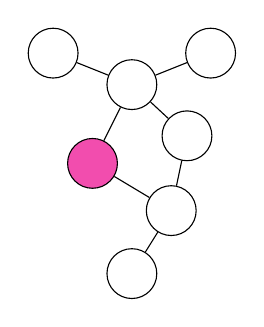
\begin{tikzpicture}
  \tikzstyle{node}=[circle,draw, minimum width=18pt, inner sep=0pt, fill=white]
  \tikzstyle{root}=[fill=magenta!70]

  \node[node, root] (1) at (0,    0)    {};
  \node[node]       (2) at (0.5,  1)    {};
  \node[node]       (3) at (1,    -0.6) {};
  \node[node]       (4) at (1.2,  0.35) {};
  \node[node]       (5) at (1.5,  1.4)  {};
  \node[node]       (6) at (-0.5, 1.4)  {};
  \node[node]       (7) at (0.5,  -1.4) {};

  \path (1) edge (2);
  \path (1) edge (3);
  \path (2) edge (4);
  \path (2) edge (5);
  \path (2) edge (6);
  \path (3) edge (4);
  \path (3) edge (7);
\end{tikzpicture}
}
\hspace{1cm}
  \subfigure[Distanz]{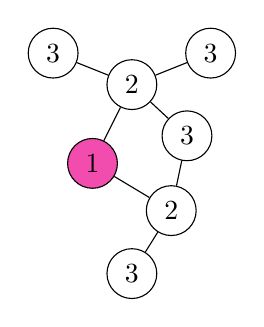
\begin{tikzpicture}
  \tikzstyle{node}=[circle,draw, minimum width=18pt, inner sep=0pt, fill=white]
  \tikzstyle{root}=[fill=magenta!70]

  \node[node, root] (1) at (0,    0)    {$1$};
  \node[node]       (2) at (0.5,  1)    {$2$};
  \node[node]       (3) at (1,    -0.6) {$2$};
  \node[node]       (4) at (1.2,  0.35) {$3$};
  \node[node]       (5) at (1.5,  1.4)  {$3$};
  \node[node]       (6) at (-0.5, 1.4)  {$3$};
  \node[node]       (7) at (0.5,  -1.4) {$3$};

  \path (1) edge (2);
  \path (1) edge (3);
  \path (2) edge (4);
  \path (2) edge (5);
  \path (2) edge (6);
  \path (3) edge (4);
  \path (3) edge (7);
\end{tikzpicture}
}
\hspace{1cm}
  \subfigure[Zentralität]{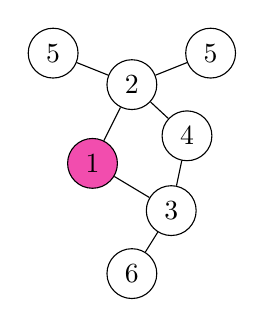
\begin{tikzpicture}
  \tikzstyle{node}=[circle,draw, minimum width=18pt, inner sep=0pt, fill=white]
  \tikzstyle{root}=[fill=magenta!70]

  \node[node, root] (1) at (0,    0)    {$1$};
  \node[node]       (2) at (0.5,  1)    {$2$};
  \node[node]       (3) at (1,    -0.6) {$3$};
  \node[node]       (4) at (1.2,  0.35) {$4$};
  \node[node]       (5) at (1.5,  1.4)  {$5$};
  \node[node]       (6) at (-0.5, 1.4)  {$5$};
  \node[node]       (7) at (0.5,  -1.4) {$6$};

  \path (1) edge (2);
  \path (1) edge (3);
  \path (2) edge (4);
  \path (2) edge (5);
  \path (2) edge (6);
  \path (3) edge (4);
  \path (3) edge (7);
\end{tikzpicture}
}
\hspace{0.6cm}
  \subfigure[Kanonisierung]{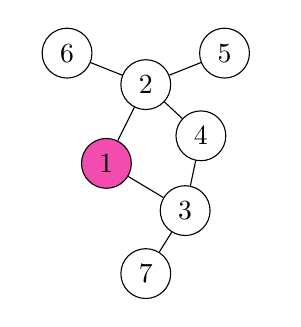
\begin{tikzpicture}
  \fill [white] (-1, 0) rectangle (2, 1) node {};  % Zentriere Graph.
  \tikzstyle{node}=[circle,draw, minimum width=18pt, inner sep=0pt, fill=white]
  \tikzstyle{root}=[fill=magenta!70]

  \node[node, root] (1) at (0,    0)    {$1$};
  \node[node]       (2) at (0.5,  1)    {$2$};
  \node[node]       (3) at (1,    -0.6) {$3$};
  \node[node]       (4) at (1.2,  0.35) {$4$};
  \node[node]       (5) at (1.5,  1.4)  {$5$};
  \node[node]       (6) at (-0.5, 1.4)  {$6$};
  \node[node]       (7) at (0.5,  -1.4) {$7$};

  \path (1) edge (2);
  \path (1) edge (3);
  \path (2) edge (4);
  \path (2) edge (5);
  \path (2) edge (6);
  \path (3) edge (4);
  \path (3) edge (7);
\end{tikzpicture}
}
\caption[Normalisierung]{Illustration der Normalisierung einer Nachbarschaft eines Knotens (rot) mit $7$ Knoten (a) zur Bestimmung einer eindeutigen Anordnung dieser.
Dazu werden die Nachbarschaftsknoten zuerst auf Basis ihrer Distanz zum Wurzelknoten gruppiert (b).
Innerhalb einer Gruppierung werden die Knoten auf Basis einer gegebenen Zentralitätsmetrik sortiert (c).
Im Anschluss werden Äquivalenzen in der Zentralität innerhalb einer Gruppe über dessen kanonische Ordnung aufgelöst (d).
Gegebenenfalls muss die gefundene Ordnung auf die gewünschte Größe des Receptive-Fields zugeschnitten oder um Fakeknoten erweitert werden.}
\label{fig:raeumliche_faltung}
\end{figure}


Nodes of any two graphs should have similar position in the
adjacency matrices iff their structural roles are similar

Canonalisierung wird nur benutzt im Ties zu brechen, damit ist der Aufwand zu vernachlässigen mit der Vorraussetzung, dass nur wenige Äquivalenzen aufgelöst werden müssen.

awdawd
